\section{Results}

The Figure below displays the results of two neural networks, one with TanH layers and one with ReLu layers, with the following parameters:
$2$ inputs, $2$ outputs and $3$ hidden layers of $25$ neurons each, $200$ epochs, a batch size of $1$ and a learning rate of $0.02$. 
The training set consists of $1000$ random 2D points between $0$ and $1$.
They are classified with a $1$ if the point is in a circle centered in $[0.5,0.5]$ and of radius equal to $1/\sqrt{2\pi}$ and $0$ when the point is outside. 
A seed is used to ensure the random generation of the parameters, in order to have reproducible initializations for debug purposes. 
The complete code is available in the Appendix~\ref{app::code}.

\begin{figure}[H]
	\begin{subfigure}[h]{0.4\textwidth}
		\begin{center}
			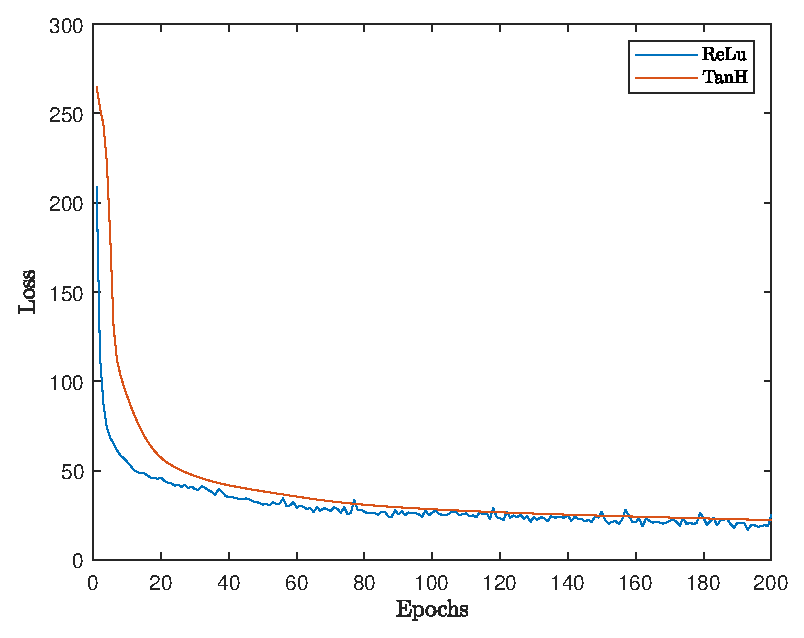
\includegraphics[width=\textwidth]{loss200}
			\caption{Loss}
		\end{center}
	\end{subfigure}
	\begin{subfigure}[h]{0.4\textwidth}
		\begin{center}
			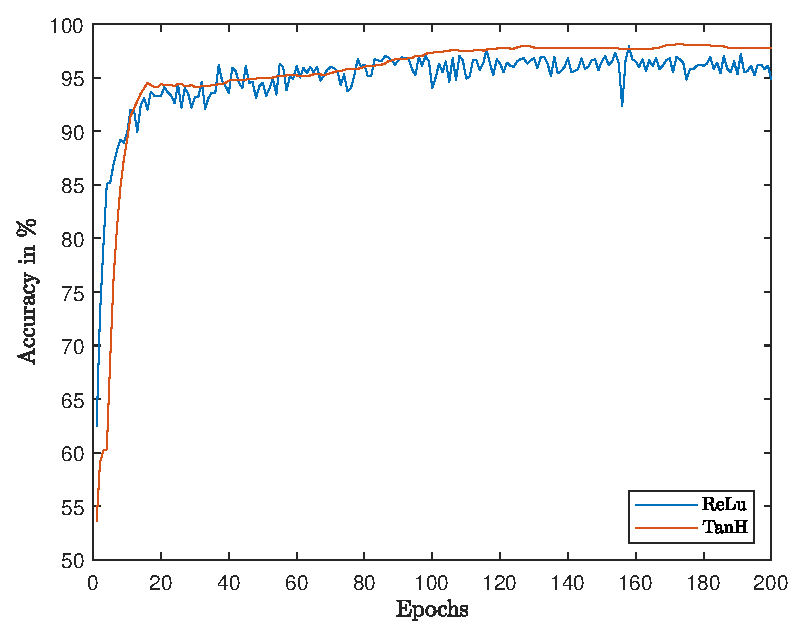
\includegraphics[width=\textwidth]{accuracy200}
			\caption{Accuracy}
		\end{center}
	\end{subfigure}
	\begin{subfigure}[h]{0.4\textwidth}
		\begin{center}
			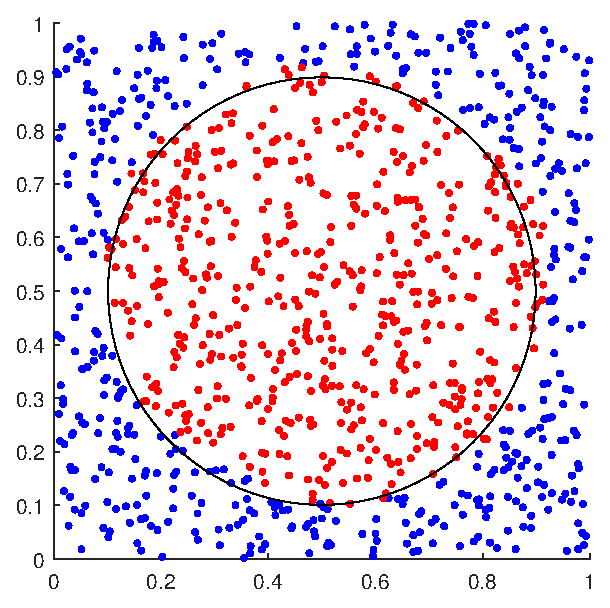
\includegraphics[width=\textwidth]{relu_out}
			\caption{Test set classified with ReLu}
		\end{center}
	\end{subfigure}
	\begin{subfigure}[h]{0.4\textwidth}
		\begin{center}
			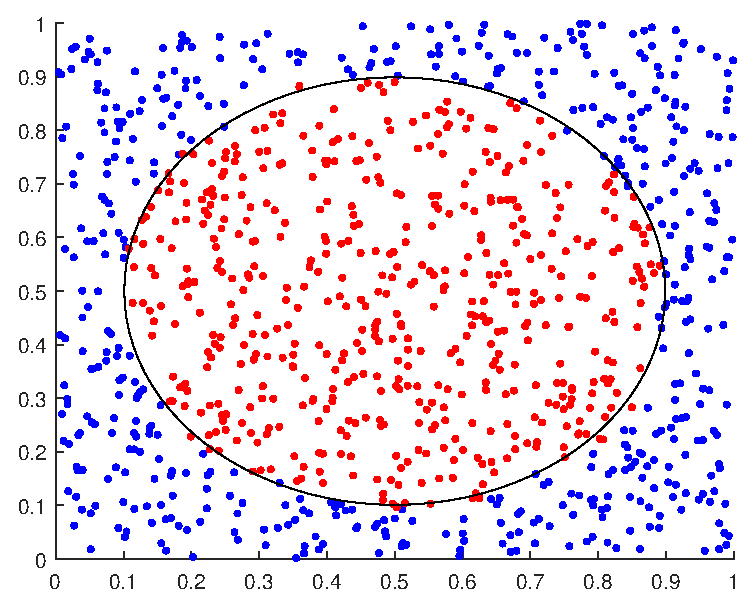
\includegraphics[width=\textwidth]{tanh_out}
			\caption{Test set classified with TanH}
		\end{center}
	\end{subfigure}
	\caption{Result of two neural networks with ReLu and TanH layers with the following parameters : $2$ inputs, $2$ outputs and $3$ hidden layers of $25$ neurons each, $200$ epochs, a batch size of $1$ and a learning rate of $0.02$.}
	\label{img::result}
\end{figure}

The final error rate for the ReLu neural network with the test set is $5.8\%$, and is $2.2\%$ with the TanH neural network.